In this chapter, the two major stochastic processes---energy straggling and multiple scattering---are detailed. Because there are so many models for these two key processes, two case studies are shown as a frame for their derivations. Both of these codes use particle-by-particle propagation and do not use the transfer map method discussed in Section~\ref{sec:cosy}.

The first case study is ICOOL \cite{icool} and covers the classic models. Much of the classic theory is also used in the new COSY routines. Consequently, the sections concerning ICOOL serve as a foundation for the derivations in Chapter \ref{chp:cosy}. ICOOL was created at Brookhaven National Laboratory for the benefit of the members of the Neutrino Factory and Muon Collider Collaboration, who specifically study ionization cooling problems.

The second case study is G4Beamline \cite{g4bl}, which is based on GEANT4 \cite{geant4}. GEANT4 implements a more novel approach. Many of the routines use empirically-tuned parameters. Consequently, G4Beamline is accurate for a variety of particles over a wide range of energies. It should be noted that muons, for which there is little experimental data available, are usually grouped with protons as heavy charged particles. Therefore, for lack of experimental data, muons use the same routines as protons.

\Section{Energy Straggling in ICOOL} \label{sec:ICOOLStraggling}\par
ICOOL \cite{icool} employs four straggling models, three of which were used in these muon simulations studies. Discussed below, these are
\begin{enumerate}
\item{Gaussian (Bohr)},
\item{Landau distribution}, and
\item{Vavilov distribution (with appropriate limits)}.
\end{enumerate}
The fourth model was not considered for this study.

\Subsection{Gaussian (Bohr) Straggling Model} \label{ssc:ICOOLStragglingGaussian}
The first model uses a Gaussian function to model the energy loss distribution. Recall that Gaussian distributions are defined by two parameters: the standard deviation $\sigma$ and the mean $\mu$. 

According to \cite{geant4}, the first of these is given by:
\begin{equation}\label{eqn:bohrvariance}
\sigma^2=2\pi e^2 N_A T_c \frac{Z\rho L}{A} \frac{1-\beta^2/2}{\beta},
\end{equation}
where $e$ is the fundamental electric charge, $N_A$ is Avagadro's number, $T_c$ is the cut kinetic energy of $\delta$-electrons, $Z$ is the nuclear charge, $\rho$ is the density of the material, $L$ is the length of the material, $A$ is the nuclear mass, and $\beta=v/c$ is the relativistic speed.

The mean comes from the Bethe-Bloch equation \cite{bethebloch}, which is derived here and yields Eq. \eqref{eqn:bethebloch}. The derivation is the so-called classical derivation, which takes first principles and mechanically derives an expression. The classically-derived intermediate equation is then subject to modern corrections, which account for the approximations made or phenomena neglected during the classical derivation.

%..........................................
%\vspace{24pt}
\noindent \textit{\large Classical Derivation}
%\vspace{12pt}

The process begins with a particle of charge $e$ moving through a material. It is assumed that the mass of the incoming particle is much greater than the mass of the electron since scattering is neglected in this derivation. Moreover, the electron must either be at rest and fixed into place (which is nonphysical) or the collision time of the particle and electron must be very small compared to the electron orbital time. The longitudinal ($z$) axis is aligned with the particle velocity such that $v_x=v_y=0$. The momentum transfer $\Delta p$ from the incoming particle to the orbiting electron is sought via
\begin{align*}
\Delta p =  \int_{-\infty} ^\infty F dt.
\end{align*}

The first observation is that the change in the longitudinal force on the particle is zero. This is true since the particle feels an average force ``forward'' just as much as it feels a force ``backward'' due to symmetry. Explicitly, this is equivalent to saying that $F_z(z)=-F_z(-z)$.
\iffalse




Explicitly, using Figure~\ref{fig:bethe_bloch} as a reference it can be seen that
\begin{align*}
\Delta p_z &= \int_{-\infty} ^\infty F_z dt = \int_{-\infty} ^\infty F \sin\theta \frac{dz}{v} = \int_{-\infty} ^\infty \frac{e^2}{r^2} \frac{z}{r} \frac{dz}{v}=\frac{e^2}{v} \int_{-\infty} ^\infty \frac{z}{r^3}dz,
\end{align*}
where $F$ is the electrostatic force ($e^2/r^2$) between the particle and the stationary electron, $r$ is the distance between the particle and the electron, and $v$ is the particle's velocity. Using
\begin{align*}
r=\sqrt{z^2+b^2},
\end{align*}
where $b$ is the impact parameter (the closest distance between the particle and the electron), then
\begin{align*}
\Delta p_z = \frac{e^2}{v} \int_{-\infty} ^\infty \frac{z}{(z^2+b^2)^{3/2}}dz = 0.
\end{align*}


\fi
For this reason, any change in momentum is solely due to the transverse force. Again following Figure~\ref{fig:bethe_bloch},
\begin{align*}
\Delta p &=\int_{-\infty} ^\infty F_x \ dt = \int_{-\infty} ^{\infty} F_x \frac{dz}{v} = \int_{-\infty} ^{\infty} F\cos{\theta}\frac{dz}{v},
\end{align*}
 Observe from Figure~\ref{fig:bethe_bloch} that $\cos\theta = b/r$. Then
\begin{align*}
\Delta p &= \int_{-\infty} ^{\infty} \frac{e^2}{r^2} \frac{b}{r} \frac{dz}{v} = \int_{-\infty} ^{\infty} \frac{e^2}{z^2+b^2} \frac{b}{\sqrt{z^2+b^2}} \frac{dz}{v}\\
\Delta p &= \frac{e^2 b}{v} \int_{-\infty} ^{\infty} \frac{1}{(z^2+b^2)^{3/2}}dz.
\end{align*}
By substitution of the following
\begin{align*}
z = b\tan{\theta},&\qquad dz = b\sec^2{\theta} d\theta,\\
z=-\infty\rightarrow \theta = \frac{-\pi}{2},&\qquad z=\infty \rightarrow \theta = \frac{\pi}{2}.
\end{align*}
the integral becomes
\begin{align*}
\Delta p &=\frac{e^2 b}{v}\int_{-\pi/2} ^{\pi/2} \frac{b\sec^2{\theta} d\theta}{(b^2(\tan^2{\theta}+1))^{3/2}} =\frac{e^2 b}{v}\int_{-\pi/2} ^{\pi/2} \frac{d\theta}{b^2 |\sec{\theta}|}\\
\Delta p&=\frac{2e^2}{vb}.
\end{align*}

\begin{figure}[h!]
  \centering
    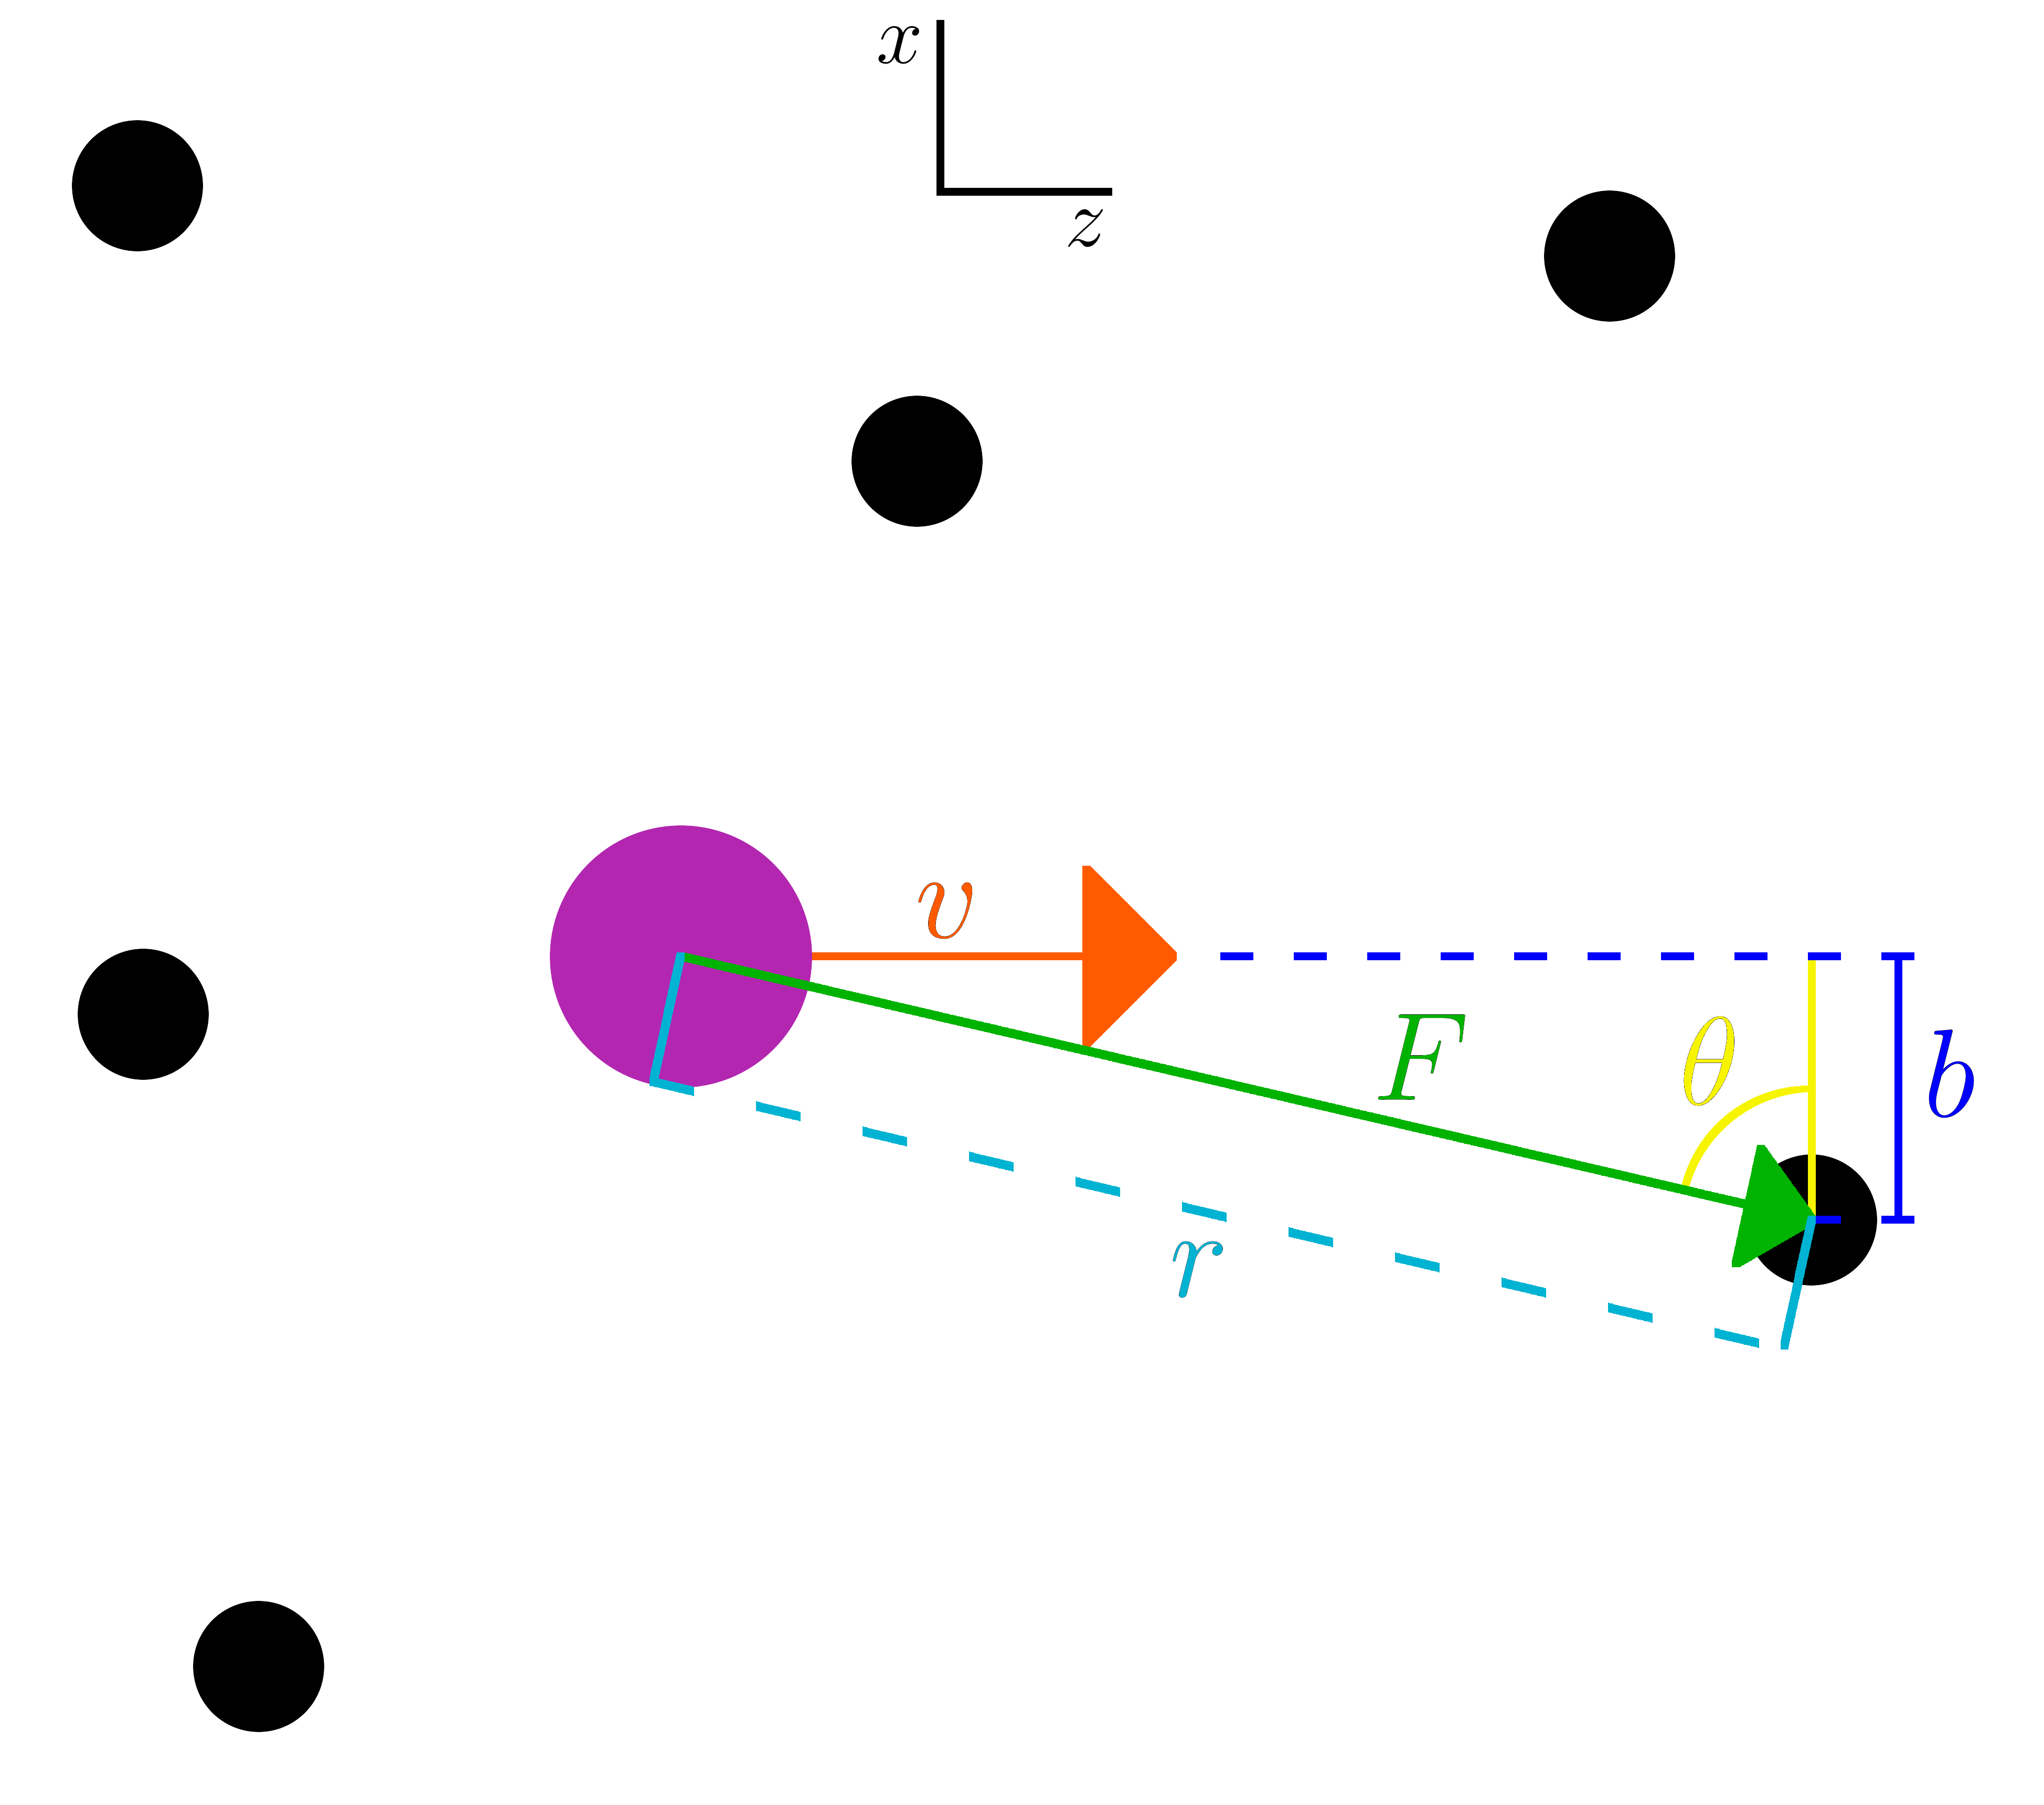
\includegraphics[width=0.7\textwidth]{Figures/bethe_bloch} 
  \caption{Classical model of particle passage through matter.}
  \label{fig:bethe_bloch}
\end{figure}

The non-relativistic approach yields the energy loss for the interaction between a muon and a single bound electron:
\begin{equation}\label{eqn:BetheBlochDeltaE}
\epsilon=\frac{\Delta p^2}{2m_e}=\frac{2e^4}{v^2 b^2 m_e}.
\end{equation}

Here, it is useful to note that if the interaction of the muon with the nucleus was desired, $\epsilon$ for a single interaction would be proportional to $Z^2/m_{nuc}$ and would be added on to Eq. \eqref{eqn:BetheBlochDeltaE}. However, since $1/m_e \gg 1/m_{nuc}$ the second term is disregarded.

Observe from Figure~\ref{fig:bethe_bloch} that only a single electron has been considered for Eq. \eqref{eqn:BetheBlochDeltaE}. For multiple electrons, the average electron density is $N_{el}=N_A\cdot Z\rho/A$, where $N_A$ is Avagadro's number, $Z$ is the nuclear charge, $\rho$ is the density of the material, and $A$ is the nuclear mass. From this expression the average energy loss may be obtained. The cylindrical symmetry of the system is exploited by integrating the single electron interaction in cylidrical coordinates, with $\theta$ as the cylindrical angle, $b$ (the impact parameter) as radius, and $z$ as length. The bounds are $\theta \in [0,2\pi]$, $z\in[0,L]$ (where $L$ is the total length of material traversed), and $b\in[b_{min},b_{max}]$ (which is discussed shortly). Then
\begin{align}
\left<\epsilon\right>&=\int_{b_{min}} ^{b_{max}} \int_0 ^L \int_0 ^{2\pi}  \frac{2e^4}{v^2b^2m_e}N_{el}\: d\theta \: dz\: b \,db \nonumber\\
&=\frac{4\pi N_A e^4}{v^2 m_e}\frac{Z\rho L}{A}\int_{b_{min}} ^{b_{max}} \frac{db}{b}. \label{eqn:BetheBlochIntermediate}
\end{align}

It is known that $b_{min}$ comes from the maximum amount of energy ($T_{max}$) which a muon may impart upon an electron. This quantity is derived later and can be seen in Eq. \eqref{eqn:tmax}, but is only symbolic here. Similarly, the minimum transferrable energy is taken as the mean ionization energy, $I$, which is usually an empirical value. Any energy below this value does not transfer, since this is the minimum amount of energy to free the electron from its orbit. Then
\begin{align*}
\epsilon_{max}&=\frac{2e^4}{v^2b_{min} ^2 m_e}=T_{max},\\
b_{min}&=\frac{e^2}{v}\sqrt{\frac{2}{m_e T_{max}}},\\[12pt]
\epsilon_{min}&=\frac{2e^4}{v^2b_{max} ^2 m_e}=T_{min}=I,\\
b_{max}&=\frac{e^2}{v}\sqrt{\frac{2}{m_e I}}.
\end{align*}

Once the bounds have been acquired, the integral in Eq. \eqref{eqn:BetheBlochIntermediate} is solvable.
\begin{align}
\left<\epsilon\right> &= \frac{4\pi N_A e^4}{v^2 m_e} \frac{Z\rho L}{A}\int_{b_{min}} ^{b_{max}} \frac{db}{b},\nonumber\\
\left<\epsilon\right> &= \frac{4\pi N_A e^4}{v^2 m_e} \frac{Z\rho L}{A} \ln{\frac{b_{max}}{b_{min}}},\nonumber\\
\left<\epsilon\right> &= \frac{2\pi N_A e^4}{v^2 m_e} \frac{Z\rho L}{A} \ln{\frac{T_{max}}{I}} \label{eqn:BetheBlochClassical}.
\end{align}

\noindent \textit{\large{Modern Corrections}}

\iffalse
While Eq. \eqref{eqn:BetheBlochClassical} is a good start, there are many aspects which were not considered. The most obvious of these are the wavelike nature of the incoming muon, relativistic kinetic energy (not simply $p^2/2m$), and the relativistic flattening of the muon's electric field just to name a few. Therefore, a more rigorous derivation is done with corrections added onto it.

Firstly, let the incoming muon be considered also a wave. Then the corresponding differential cross section $d\Sigma$ is defined as the area in which the muon loses an amount of energy between $\epsilon$ and $\epsilon+d\epsilon$. Given the impact parameter $b$, for a single electron this area is a ring of radius $b$ and thickness $db$, or \cite{bichsel1968,bichsel1988}
\begin{align*}
d\Sigma=2\pi b \, db.
\end{align*}
Using the result from Eq. \eqref{eqn:BetheBlochDeltaE} in the classical derivation, this becomes
\begin{align*}
\epsilon &= \frac{2e^4}{\beta^2 b^2 m_e}\\
b^2 &= \frac{2e^4}{\beta^2 \epsilon m_e}\\
2b \, db &= -\frac{2e^4}{\beta^2 \epsilon^2 m_e}d\epsilon,
\end{align*}
and so
\begin{align*}
d\Sigma=\frac{2\pi e^4}{\beta^2} \frac{d\epsilon}{\epsilon ^2}.
\end{align*}
The relativistic correction for this was calculated by Bhabha \cite{uehling,bhabha} and results in
\begin{align*}
d\Sigma=\frac{2\pi e^4}{\beta^2} \frac{d\epsilon}{\epsilon ^2}\Big(1-\frac{\beta^2 \epsilon}{T_{max}}\Big).
\end{align*}
Note that in \cite{uehling}, this result is only for spin-0 particles, and there is a further correction factor of $\epsilon ^2 / 2E^2$ for spin-1/2 particles. However, since $E>>\epsilon$ this term is usually ignored.

The cross section may now be used in the standard definition of moments (or expectation values). Then
\begin{align} \label{eqn:StragglingMoments}
\left< M^j\right>&=N_{el} L \int_{\epsilon_{min}} ^{\epsilon_{max}} \epsilon^j \frac{d\Sigma}{d\epsilon} d\epsilon .
\end{align}
The moments are simply equal to the expectation values as $M^j=\left<\epsilon ^j \right>$, except for $M^0$, since $\left< \epsilon ^0 \right>=\left< 1 \right> = 1$. Instead, $M^0$ is the mean number of collisions, and the actual number of collisions is sampled from a Poisson distribution with this average.

While the upper limit $\epsilon_{max}$ is still valid since it was derived explicitly from relativistic principles, the lower limit $\epsilon_{min}$ should be re-evaluated from its classical assumption. \cite{bichsel1968} points out that the incoming particle interacts with all of the electrons in the atom, not simply a single valence electron. These interactions may be significant enough to invalidate the classical model and therefore should be considered. $I$ is defined as (see for example Eqns. \ref{eqn:G4StragglingOscillatorConstraint1} and \ref{eqn:G4StragglingOscillatorConstraint2} in Section~\ref{sec:g4blstraggling})
\begin{gather*}
Z \ln I = \sum_i f_i E_i
\end{gather*}
where $f_i$ are oscillator strengths and $E_i$ are ionization energies for the $i^{th}$ level.
\fi

\iffalse
It is interesting to note that the zeroth moment is the mean number of collisions, and that the actual number of collisions is sampled from a Poisson distribution with this average. Moreover, $\left<\epsilon^1\right>$ is the mean energy loss, which is the desired outcome of this derivation. Then
\begin{align*}
\left<\epsilon\right>&=\frac{Z\rho L}{A} \frac{2\pi e^4}{\beta^2} \int_I ^{T_{max}} \frac{d\epsilon}{\epsilon} \Big(1-\frac{\beta^2 \epsilon}{T_{max}}\Big)\\
\left<\epsilon\right>&=\frac{Z\rho L}{A} \frac{2\pi e^4}{\beta^2} \Big(\ln{\frac{T_{max}}{I}}-\beta^2 (1-\frac{I}{T_{max}})\Big)
\end{align*}
\fi





There are a number of corrections to the Bethe-Bloch equation. The first is a correction under the logarithm due to the relativistic flattening of the incoming particle's electric field. This factor is  $2m_e \beta^2 \gamma^2 / I$. Another correction is known as the density correction $\delta$ and arises due to polarization of the material. This is important for high energies since it can limit the range of the flattened electric field in the material. The last correction is the shell correction $C$ and accounts for the fact that the electron is not at rest (or the interaction time is not much faster than the electron orbit). This is important for low energies. These corrections may or may not have a large impact on these medium energy studies since the logarithmic and density corrections arise at high energies and the shell correction occurs at low energies. Finally, in its more familiar form, the constants in Eq. \eqref{eqn:BetheBlochClassical} are condensed into a single constant $K=\frac{2\pi e^4 N_A}{m_e}\approx 15.4$ $ (\text{MeV}\cdot \text{cm}^3)/(\text{m}\cdot \text{g})$. Since the model assumes natural units (i.e. $c=1$), $v^2$ is usually replaced with $\beta ^2$. Moreover, to avoid confusion $\left<\epsilon\right>$ is given a negative sign in order to emphasize energy \emph{loss}.

The ultimate result is the Bethe-Bloch equation for the average energy lost by a particle traversing some medium with correction factors:
\begin{equation}\label{eqn:bethebloch}
\left< \epsilon \right> = -\frac{K}{\beta^2}\frac{Z\rho L}{A}\Big(\ln{\frac{2m_e \beta ^2 \gamma ^2 T_{max}}{I^2}}-2\beta^2-\delta-2\frac{C}{Z}\Big).
\end{equation}

According to the Particle Data Group \cite{PDG}, this equation is generally accurate for intermediate $Z$ materials (up to a few \% when compared to experimental data) in the energy regime of $0.1 \lesssim \beta \gamma \lesssim 1000$. The lower limit of this equation is reached when the incoming particle velocity is comparable to the atomic electron velocities and the upper limit is attained due to radiative effects, and both limits exhibit some $Z$ dependence. Figure~\ref{fig:bethecurve} depicts this region with muons on copper. Clearly, the region typically used for muon ionization cooling ($100 \text{ MeV/}c < p_\mu < 1000 \text{ MeV/}c$) falls in the middle of the Bethe region.

%..........................................
\vspace{24pt}
\noindent \textit{\large{Derivation of $\,T_{max}$}}
\vspace{12pt}

Although $T_{max}$ is used symbolically in many equations, here it is derived explicitly from a relativistic point of view. This derivation yields Eq. \eqref{eqn:tmax} and works in natural units such that $c=1$. Conservation of energy for a muon incident upon an electron at rest requires that 
\begin{align}
E_\mu+m_e&=E_{\mu,f}+E_e,&\text{ or} \nonumber\\
\sqrt{p_\mu ^2+m_\mu ^2}+m_e &= \sqrt{p_{\mu,f}^2+m_\mu ^2}+T_e+m_e,&\text{ or} \nonumber \\
p_{\mu,f}^2 =p_\mu^2 &+T_e^2-2T_e\sqrt{p_\mu ^2 + m_\mu^2}, \label{eqn:TMaxEnergy1}
\end{align}
with
\begin{align}
E_e=T_e&+m_e = \sqrt{p_e ^2+m_e^2},\qquad\text{ or} \nonumber\\
p_e ^2&=(T_e+m_e)^2-m_e^2, \label{eqn:TMaxEnergy2}
\end{align}
where $T_e$ is the final kinetic energy of the electron, $p_\mu$ is the initial muon momentum, $m_\mu$ is the mass of the muon, and $p_{\mu,f}$ is the final muon momentum. 

Conservation of momentum requires that
\begin{align*}
\vec{p}_\mu&=\vec{p}_{\mu,f}+\vec{p}_e, \qquad\text{ or}\\
 p_{\mu,f}^2&=p_\mu ^2 + p_e^2-2p_\mu p_e \cos\alpha,
\end{align*}
where $\alpha$ is the angle between the initial muon momentum and the final electron momentum.
Using Eq. \eqref{eqn:TMaxEnergy2} for $p_e$ on the right-hand side this becomes
\begin{align*}
p_{\mu,f}^2=p_\mu ^2+(T_e+m_e)^2-m_e ^2-2p_\mu\cos\theta \sqrt{(T_e+m_e)^2-m_e^2}.
\end{align*}
Now subsitution of Eq. \eqref{eqn:TMaxEnergy1} for $p_{\mu,f} ^2$ on the left-hand side yields
\begin{align*}
p_\mu ^2+T_e ^2 - 2T_e \sqrt{p_\mu^2+m_\mu ^2}&=p_\mu ^2+(T_e+m_e)^2-m_e ^2 -2p_\mu\cos\theta\sqrt{(T_e+m_e)^2-m_e^2}.
\end{align*}
For maximum energy (i.e. to attain $T_e=T_{max}$), $\cos\theta=1$, which is representative of a head-on collision. Then
\begin{align*}
T_{max} ^2-2T_{max}\sqrt{p_\mu ^2+m_\mu ^2} &=T_{max}^2+2T_{max}m_e-2p_\mu\sqrt{T_{max}^2+2T_{max}m_e}\\
-2T_{max}(\sqrt{p_\mu ^2 + m_\mu ^2}+m_e)&=-2p_\mu\sqrt{T_{max}^2+2T_{max}m_e}\\
\sqrt{p_\mu ^2+m_\mu ^2}+m_e&=p_\mu\sqrt{1+\frac{2m_e}{T_{max}}}.
\end{align*}
Substituting the initial muon energy $E_\mu=\sqrt{p_\mu ^2+m_\mu ^2}=\gamma m_\mu$ and the initial muon momentum $p_\mu ^2=E_\mu ^2 - m_\mu ^2 = m_\mu ^2 (\gamma^2-1)=m_\mu ^2 \gamma^2 \beta^2$ results in
\begin{align*}
\gamma m_\mu + m_e &= m_\mu\gamma\beta\sqrt{1+\frac{2m_e}{T_{max}}}\\
(\gamma m_\mu +m_e)^2 &=m_\mu^2\gamma^2\beta^2 \Big(1+\frac{2m_e}{T_{max}}\Big).
\end{align*}
Finally, solving for the maximum transferrable energy from an incident muon to an electron at rest is
\begin{equation}\label{eqn:tmax}
T_{max}=\frac{2m_e \beta^2 \gamma^2}{1+2\gamma\frac{m_e}{m_\mu}+(\frac{m_e}{m_\mu})^2}.
\end{equation}

%-----------------------------------------------------------------------------------------------------------
\Subsection{Landau Straggling Model}\label{ssc:ICOOLStragglingLandau}

The second ICOOL straggling model selects an energy loss from a Landau distribution \cite{landau}. This derivation is particularly important since it is the same model that was implemented into COSY in this work. Landau begins the derivation by stipulating that this theory assumes fast particles (``so that the usual ionisation theory may be applied'', here taken as particles whose energy is in the Bethe regime in Figure~\ref{fig:bethecurve}). Moreover, the thickness of the absorber should be small enough, so that the energy loss is small compared to the initial energy. Landau defines the weight function $w(E,u)$ as the probability per unit length of an energy loss $u$ given the instantaneous total energy $E$. For the aforementioned constraints, the weight function may be written simply as $w(u)$ (since $E$ is now a constant instead of a variable). Another way of describing this constraint is that the total energy of the particle is roughly constant while traversing the medium.

Let $f(L,\epsilon)$ be the desired distribution function for the energy loss. This means that the particle loses an amount of energy between $\epsilon$ and $\epsilon+d\epsilon$ while traversing an absorber of length $L$. Then on one hand
\begin{align*}
\text{change in $f$ per unit length }=\frac{\partial f(L,\epsilon)}{\partial L}.
\end{align*}
On the other hand, the change in $f$ may also be expressed as the difference of two functions: one at a length $L$ with possible energy losses between $\epsilon$ and $\epsilon+d\epsilon$ and another at length $L$ and with possible energy losses between $\epsilon-u$ and $\epsilon+d\epsilon-u$, with $u$ accounting for the infinitesimal change in length. Then
\begin{align*}
\text{change in $f$ per unit length }=\Bigg [\int_0 ^\infty w(u) f(L,\epsilon-u) du \Bigg] - f(L,\epsilon).
\end{align*}
Often referred to as the integral transport equation, the two previous definitions of the change in $f$ per unit length may be combined as
\begin{align}\label{eqn:Landau1}
\frac{\partial f(L,\epsilon)}{\partial L} = \Bigg [\int_0 ^\infty w(u) f(L,\epsilon-u) du \Bigg] - f(L,\epsilon).
\end{align}
Since $L$ and $\epsilon$ are independent and implicit variables, this allows for a Laplace transformation. Take the transformed function with respect to $\epsilon$ as 
\begin{align*}
\phi(p,L)=\int_0 ^\infty e^{-p \epsilon} f(\epsilon) d\epsilon.
\end{align*}
(Note that $p$ is simply a dummy variable and not the momentum.)
%
Then the inverse transformation gives
\begin{align} \label{eqn:LandauInverseTransformation}
f(L,\epsilon)=\frac{1}{2\pi i} \int_{K-i \infty} ^{K+i\infty} \phi(p,L) e^{p\epsilon} dp.
\end{align}
Observe here that $K>0$ and so the integral is just to the right of the imaginary axis. This is the desired distribution function, and so is useful later. However, without the form of $\phi$ it is not useful. The goal then is to find a closed form of $\phi$.

Multiplying both sides of Eq. \eqref{eqn:Landau1} by $e^{-p\epsilon}$ and integrating with respect to $d\epsilon$ yields
\begin{align*}
\int_0 ^\infty \frac{\partial f}{\partial L} e^{-p\epsilon} d\epsilon = \int_0 ^\infty \Bigg [\int_0 ^\infty w(u) f(L,\epsilon-u) du \Bigg]e^{-p\epsilon} d\epsilon -  \int_0 ^\infty f(L,\epsilon) e^{-p\epsilon} d\epsilon.
\end{align*}
On the left side, the operations of partial derivative and integration are commutable, and are therefore switched. On the right side, the first term has commutable integrations and so the order is switched. For the second term, note that $w(u)$ is normalized, so adding the integral of $w(u)$ over all $u$ changes nothing. Dropping the implicit $L$ for now,
\begin{align*}
\frac{\partial}{\partial L}\int_0 ^\infty e^{-p\epsilon} f(\epsilon) d\epsilon = &\int_0 ^\infty \Bigg[\int_0 ^\infty e^{-p\epsilon} f(\epsilon-u)  d\epsilon \Bigg] w(u) du -\\
 & \int_0 ^\infty \Bigg[\int_0 ^\infty e^{-p\epsilon}f(\epsilon) d\epsilon \Bigg] w(u) du.
\end{align*}
Parts of the left side and the second term on the right side may be substituted for $\phi$ directly, while the first term on the right side should be shifted by $-u$, resulting in
\begin{align*}
\frac{\partial}{\partial L} \phi(p,L) &= \int_0 ^\infty \Bigg[\int_{-u} ^\infty e^{-p(\epsilon+u)} f(\epsilon)  d\epsilon \Bigg] w(u) du -\int_0 ^\infty \phi(p,L) w(u) du.
\end{align*}
Now recall that $f(\epsilon)$ is the desired function for energy loss. Therefore, $f(\epsilon<0)=0$ (i.e. the particle cannot gain energy while traversing a medium), and so
\begin{align}
\frac{\partial}{\partial L} \phi(p,L) &= \int_0 ^\infty e^{-pu}\Bigg[\int_{0} ^\infty e^{-p\epsilon} f(\epsilon)  d\epsilon \Bigg] w(u) du -\phi(p,L) \int_0 ^\infty w(u) du\nonumber\\
&=\phi(p,L)\int_0 ^\infty w(u)(e^{-pu}-1)\, du. \nonumber%\label{eqn:LandauPhiDifferentialEquation}
\end{align}

This differential equation is a first-order, undriven normal linear ODE (ordinary differential equation) \cite{Borrelli}. Let prime ( $'$ ) denote a partial derivative with respect to $L$. Then the strategy to solve this ODE is to define a function $h(L)$ as
%
\begin{gather*}
h(L)=-\int_0 ^\infty w(u)  (e^{-pu}-1)\, du
\end{gather*}
and its antiderivative as
\begin{gather*}
H(L)=\int h(L) dL=L \int_0 ^\infty w(u)  (1-e^{-pu})\, du.
\end{gather*}
Then
\begin{equation}\label{eqn:landauODE}
\phi ' + \phi \cdot h(L) = 0.
\end{equation}
%
Since $(e^{H(L)}) ' = e^{H(L)}\cdot H'(L)= e^{H(L)}\cdot h(L)$ , it is useful to multiply both sides of the ODE in Eq. \eqref{eqn:landauODE} by $e^{H(L)}$, resulting in
\begin{gather*}
\phi ' \cdot e^{H(L)}+ \phi \cdot h(L) \cdot e^{H(L)} = 0,\\
(\phi\cdot e^{H(L)}) ' = 0.
\end{gather*}
Integrating both sides yields
\begin{gather*}
\phi\cdot e^{H(L)}=K_1,\\
\phi = K_1 e^{-H(L)},\\
\phi(p,L)=K_1 \exp\Big[-L\int_0 ^\infty w(u)  (1-e^{-pu})\, du\Big].
\end{gather*}

This differential equation is now solvable provided that there are initial conditions. The first observation is that for $L=0$, the only possible energy loss is zero. Mathematically, this means that $f(0,\epsilon)=\delta(\epsilon)$; that is, the probability of energy loss is 100\% for an energy loss of zero and 0\% for all other energy losses. Then the boundary condition on $\phi$ is
\begin{align}
\phi(p,0)&=\int_0 ^\infty \delta(\epsilon) e^{-p\epsilon}\, d\epsilon\nonumber\\
\phi(p,0)&=e^{p\cdot 0}\nonumber\\
\phi(p,0)&=1=K_1\exp[0].\nonumber%\label{eqn:LandauPhiInitialCondition}
\end{align}
Then
\begin{gather*}
\phi(p,L)=\exp\Big[-L\int_0 ^\infty w(u)  (1-e^{-pu})\, du\Big].
\end{gather*}

Now using Eq. \eqref{eqn:LandauInverseTransformation}, the energy loss distribution function $f$ in terms of $w(u)$ is 
\begin{equation} \label{eqn:LandauGeneralSolution}
f(L,\epsilon)=\frac{1}{2\pi i} \int_{K-i\infty} ^{K+i\infty} \exp\Big[p\epsilon-L\int_0 ^\infty w(u)  (1-e^{-pu})\, du\Big] dp.
\end{equation}
In principle, this is the general solution to the energy loss profile for a particle traversing some medium. In practice, the only thing which is inhibiting implementation is an algorithm to generate a number from this distribution (which is discussed in Chapter \ref{chp:cosy}) and the function $w(u)$. Once $w(u)$ is obtained, the integral may be found using numeric integration, provided that it is not computationally expensive.

Livingston and Bethe \cite{livingston} derived the form of $w(u)$ in 1937, and it is
\begin{align*}
w(u)&=\frac{\xi}{L}\frac{1}{u^2},
\end{align*}
where
\begin{equation}\label{eqn:xi}
\xi=\frac{2\pi r_e ^2 m_e N_A Z\rho L}{\beta^2 A}
\end{equation}
and $r_e$ is the classical electron radius, $m_e$ is the electron mass, $N_A$ is Avagadro's number, $Z$ is the nuclear charge, $\rho$ is the density of the material, $L$ is the length of the material, $A$ is the nuclear mass, and $\beta=v/c$ is the relativistic speed. Now the form of $w(u)(1-e^{-pu})$ may be seen in Figure~\ref{fig:landauPUPlot}. It can be seen that the most important values of $p$ are those where $pu \ll 1$ and $1 \ll pu$ since values of $pu\approx 1$ tends to vanish.

\begin{figure}[h!]
  \centering
    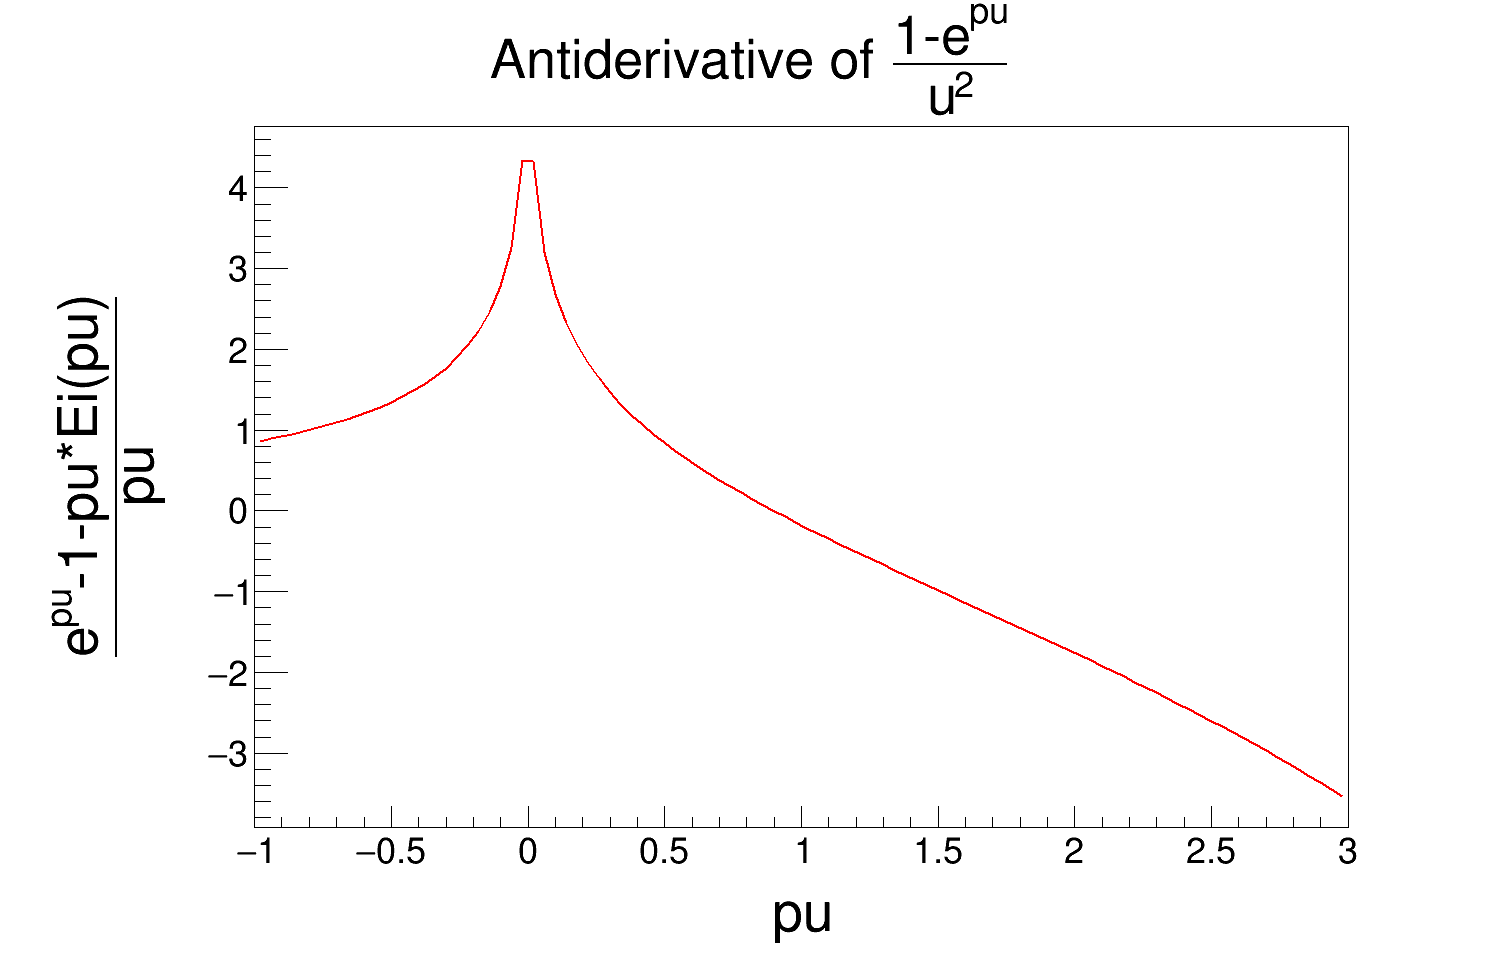
\includegraphics[width=0.7\textwidth]{Figures/landauPUPlot} 
  \caption[Plot of $\int w(u)(1-e^{-pu})\ du$.]{Plot of $\int w(u)(1-e^{-pu})\ du$ for various $pu$. On the vertical axis is the antiderivative of $w(u)(1-e^{-pu})$, with $\text{Ei}(x)$ representing the exponential integral.}
  \label{fig:landauPUPlot}
\end{figure}

Rather than zero, let $u_{min}$ be the minimum possible energy loss. Now consider a certain energy $u_1$ such that $u_{min}\ll u_1$ and $pu_1 \ll 1$. Then the integral in the exponent of Eq. \eqref{eqn:LandauGeneralSolution} has the form
\begin{align*}
L\int_0 ^\infty w(u)  (1-e^{-pu})\, du &= \xi\Big( \int_0 ^{u_1} \frac{1-e^{-pu}}{u^2} du + \int_{u_1} ^\infty \frac{1-e^{-pu}}{u^2} du\Big) .
\end{align*}
Since the first integral is over the small values, it is possible to write $1-e^{pu} \approx 1-(1-pu) = pu$. Furthermore, the minimum energy loss is not 0 but rather $u_{min}$. Then
\begin{align*}
\frac{L}{\xi}\int_0 ^\infty w(u)  (1-e^{-pu})\, du &=\int_{u_{min}} ^{u_1} \frac{p\ u}{u^2} du + \int_{u_1} ^\infty \frac{1-e^{-pu}}{u^2} du\\
&=p\int_{u_{min}} ^{u_1} \frac{1}{u} du + \int_{u_1} ^\infty \frac{1-e^{-pu}}{u^2} du\\
&=p \ln\frac{u_1}{u_{min}} + \int_{u_1} ^\infty \frac{1-e^{-pu}}{u^2} du.
\end{align*}
For the second term, integration by parts and evaluation at the boundaries gives
\begin{align*}
\frac{L}{\xi}\int_0 ^\infty w(u)  (1-e^{-pu})\, du &=p \ln\frac{u_1}{u_{min}} + \frac{1-e^{-pu_1}}{u_1}+p\int_{u_1}^\infty \frac{e^{-pu}}{u} du.
\end{align*}
Recalling that $u_1$ was chosen such that $pu_1 \ll 1$, the exponential in the second term may be approximated as $e^{-pu_1}\approx 1-pu_1$. Then
\begin{equation} \label{eqn:landauIntermediate1}
\frac{L}{\xi}\int_0 ^\infty w(u)  (1-e^{-pu})\, du =p \ln\frac{u_1}{u_{min}} + p+p\int_{u_1}^\infty \frac{e^{-pu}}{u} du.
\end{equation}
The final integral may be evaluated first by letting $K_2=pu$:
\begin{align*}
\frac{L}{\xi}\int_{u_1}^\infty \frac{e^{-pu}}{u} du &= \int _{pu_1} ^\infty \frac{e^{-K_2}}{K_2}dK_2\\
&= \int_{pu_1} ^\infty \frac{e^{-K_2}}{K_2} dK_2 + \int_{pu_1} ^1 \frac{dK_2}{K_2} - \int_{pu_1} ^1 \frac{dK_2}{K_2} \\
&= \int_{pu_1} ^1 \frac{e^{-K_2}}{K_2} dK_2 + \int_1 ^\infty \frac{e^{-K_2}}{K_2} dK_2 + \int_{pu_1} ^1 \frac{dK_2}{K_2} - \int_{pu_1} ^1 \frac{dK_2}{K_2} \\
&= \int_{pu_1} ^1 \Big(\frac{e^{-K_2}}{K_2}-\frac{1}{K_2}\Big) dK_2 + \int_1 ^\infty \frac{e^{-K_2}}{K_2} dK_2 + \int_{pu_1} ^1 \frac{dK_2}{K_2} \\
&= \int_{pu_1} ^1 \frac{dK_2}{K_2} + \left[\int_{pu_1} ^1 \frac{e^{-K_2}-1}{K_2} dK_2 + \int_1 ^\infty \frac{e^{-K_2}}{K_2} dK_2 \right].
\end{align*}
The first term is easily evaluated, and the second term in brackets is approximately\footnote{This expression would be exactly $-C_{Euler}$ if $pu_1=0$.} the negative of Euler's constant, $-C_{Euler}$. Putting this back into Eq. \eqref{eqn:landauIntermediate1} yields
\begin{align*}
\frac{L}{\xi}\int_0 ^\infty w(u)  (1-e^{-pu})\, du &=p \ln\frac{u_1}{u_{min}} + p(1-C_{Euler}-\ln pu_1)\\
&=p(1-C_{Euler}-\ln pu_{min}).
\end{align*}

Now Eq. \eqref{eqn:LandauGeneralSolution} may be rewritten as
\begin{align*}
f(L,\epsilon)&=\frac{1}{2\pi i} \int_{K-i\infty} ^{K+i\infty} \exp\Big[p\epsilon-L\int_0 ^\infty w(u)  (1-e^{-pu})\, du\Big] dp\\
&= \frac{1}{2\pi i} \int_{K-i\infty} ^{K+i\infty} \exp\Big[p\epsilon-p\xi(1-C_{Euler}-\ln pu_{min})\Big] dp.
\end{align*}
If a unitless variable of integration is desired, then $p\rightarrow p/\xi$, and
\begin{align*}
f(\xi,\epsilon)&=\frac{1}{2\pi i \xi} \int_{K-i\infty} ^{K+i\infty} \exp\Big[p\frac{\epsilon}{\xi}-p(1-C_{Euler}-\ln \frac{u_{min}}{\xi})+p\ln p\Big] dp,
\end{align*}
or simply
\begin{equation}\label{eqn:landau}
f(\lambda)=\frac{1}{2\pi i \xi} \int_{K-i\infty} ^{K+i\infty} \exp\Big[p\ln p + \lambda p\Big] dp,
\end{equation}
where evidently
\begin{align*}
\lambda = \frac{\epsilon}{\xi} -1+C_{Euler}+\ln \frac{\xi}{u_{min}}.
\end{align*}
However, typically the Landau function is evaluated for the desired \emph{fluctuation about the mean energy loss}, not the energy loss itself. Because of this, $\lambda$ must be shifted by the mean, $\left< \epsilon \right>$. Furthermore, a relativistic correction of $-\beta ^2$ is added and $u_{min}\rightarrow T_{max}$ (from Eq. \eqref{eqn:tmax}), resulting in the final form of the Landau parameter:
\begin{equation}\label{eqn:landauParameter}
\lambda \equiv \frac{\epsilon-\left<\epsilon\right>}{\xi}-(1-C_{Euler})-\beta ^2 -\ln (\xi/T_{max}).
\end{equation}

\begin{figure}[h!]
  \centering
    \includegraphics[width=0.7\textwidth]{"Figures/landau example"} 
  \caption[Example of the Landau function.]{Example of the Landau function.}
  \label{fig:landau_example}
\end{figure}

In summary, the ICOOL Landau model uses the mean energy loss from the Bethe-Bloch equation (Eq. \eqref{eqn:bethebloch}). The routine then adds noise based on the Landau function (see, e.g., Figure~\ref{fig:landau_example}), which has a mode of zero. This value is then accepted as the total energy loss of the particle.

%-------------------------------------------------------------------------------
\Subsection{Vavilov Straggling Model}\label{sec:ICOOLVavilov}\par
The Vavilov model \cite{vavilov} is similar to the Landau model, except that the thickness of the absorber is not required to be small enough such that the energy loss is small compared to the initial energy. The derivation is also similar, except that Vavilov introduced a limit on the maximum transferable energy due to a single collision (recall that in Landau theory the upper limit was $\infty$). The result is
\begin{equation}\label{eqn:vavilov}
f(\lambda_v, \kappa, \beta^2)=\frac{1}{\xi}\phi_v (\lambda_v , \kappa, \beta^2),
\end{equation}
where
\begin{align*}
\phi_v (\lambda_v,\kappa,\beta^2)&=\frac{1}{2\pi i}\int_{K+i\infty} ^{K-i\infty} \phi(p,\kappa,\beta^2) e^{\lambda p},\\
\phi(p,\kappa,\beta^2)&=\exp[\kappa(1+\beta^2 \gamma)]\exp[\psi(p,\kappa,\beta^2)],\\
\psi(p)&=p\ln \kappa + (p+\beta^2\kappa)[\ln(p/\kappa)+E_1 (p/\kappa)]-\kappa e^{-p/\kappa},\\
E_1 (p)&= \int_\infty ^z \frac{e^{-u}}{u} du \qquad \text{(the exponential integral)},\\
\lambda_v &= \kappa\Big(\frac{\epsilon-\left<\epsilon\right>}{\xi}-(1-C_{Euler})-\beta^2\Big)= \kappa(\lambda+\ln\kappa),\text{ and}\\
\kappa&=\xi/T_{max}.
\end{align*}
While this function in theory is universal for the needs of this study, clearly such a distribution function requires numeric methods, and as such is more costly than the Landau method. Fortunately, the Vavilov distribution converges to either the Landau distribution (for $\kappa\rightarrow 0$) or a Gaussian distribution (for $\kappa\rightarrow\infty$) at its extrema. The cutoffs for these extrema in practice are

\begin{align*}
\phi_v=
	\begin{cases}
	\text{Landau via Eq. \eqref{eqn:landau}} & \kappa\leq 0.01\\
	\text{Vavilov via Eq. \eqref{eqn:vavilov}} & 0.01 < \kappa < 10\\
	\text{Gaussian via }Gaus(\left<\epsilon\right>,\sigma)\text{ in Eqns. \ref{eqn:bethebloch} and \ref{eqn:bohrvariance}} & 10\leq\kappa
	\end{cases}.
\end{align*}

%=================================================================================
\Section{Multiple Scattering in ICOOL} \label{sec:ICOOLScattering} \par
ICOOL version 3.30 \cite{icool} boasts a total of seven models of multiple scattering:
\begin{enumerate}
\item Gaussian ($\sigma$ determined by Rossi-Greisen model),
\item Gaussian ($\sigma$ determined by Highland model),
\item Gaussian ($\sigma$ determined by Lynch-Dahl model),
\item Bethe version of Moli\`{e}re distribution with Rutherford limit,
\item Rutherford,
\item Fano with Rutherford limit, and
\item Tollestrup with Rutherford limit.
\end{enumerate}
The scattering model used in this work is Fano with Rutherford limit, which is also the default scattering model in ICOOL. The following is a derivation of the Rutherford model accompanied by a brief discussion of the Fano model. Unless otherwise stated, the derivation of the Rutherford model closely follows \cite{griffithsqm}.

The Rutherford model is used in part in four out of the seven models because it is so robust. The derivation can be done using the Coulomb potential, classical mechanics, the Born approximation, and quantum field theory, with the quantum mechanics Born approximation being the weapon of choice here. Recall that the quantum model used in this work is represented by Figure~\ref{fig:qmscatteringmodel}.
\begin{figure}
  \centering
    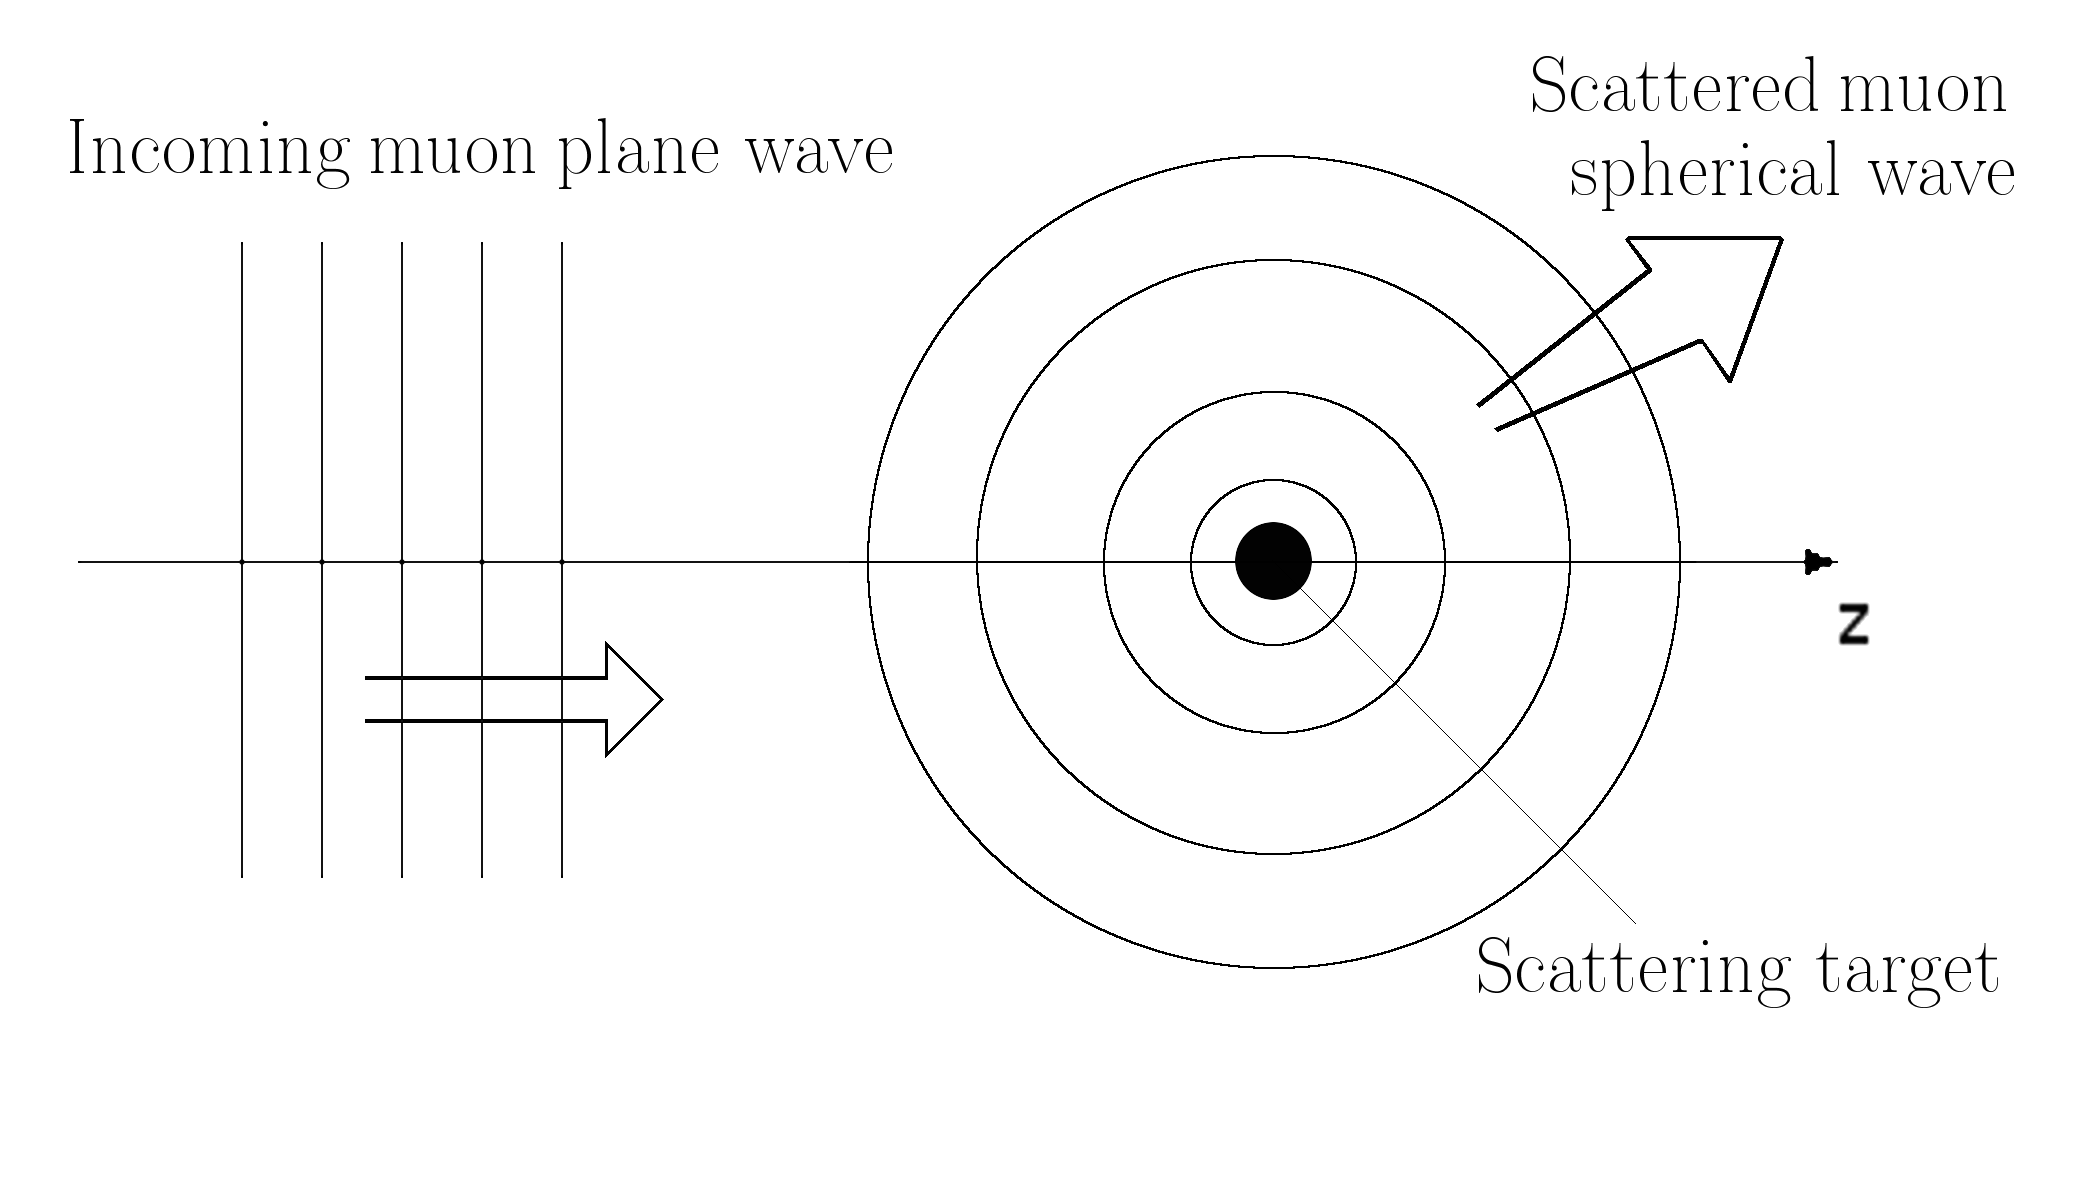
\includegraphics[width=\textwidth]{Figures/scattering_model_2} 
  \caption{Quantum scattering model.}
  \label{fig:qmscatteringmodel}
\end{figure}
Here there is an incoming plane wave (mathematically represented by $e^{ikz}$) and a spherical wave (represented by $e^{ikr}/r$). $r$ and $z$ are coordinates, $i$ is the imaginary unit, and $k$ is the wave number, classically related to the energy as $k=\sqrt{2mE}/\hbar$. Then basic quantum mechanics suggests that the solution to the Schr\"{o}dinger equation has the form
\begin{equation}
\label{eqn:scatteringwavefunction}
\psi (r,\theta)\approx A \left(e^{ikz}+f(\theta)\frac{e^{ikr}}{r}\right),
\end{equation}
where $A$ is the total amplitude and $f(\theta)$ is the scattering amplitude. The probability of the particle scattering in a particular direction is given by the amplitude squared, $|f(\theta)|^2$, and is the object of this derivation. Now, $\psi$ solves the differential (time-independent) Schr\"{o}dinger equation, which usually has the form
\begin{equation} \nonumber
-\frac{\hbar^2}{2m}\nabla^2\psi+V\psi=E\psi,
\end{equation}
where $V$ is the system potential and $E$ is the energy of the wavefunction. This can be expressed alternatively by assigning $Q\equiv V\psi\cdot{2m}/{\hbar^2}$ and recalling that $k=\sqrt{2mE}/\hbar$. Then
%
\begin{equation}
\label{eqn:schrodinger}
(\nabla^2+k^2)\psi=Q.
\end{equation}

The strategy is to solve Eq. \eqref{eqn:schrodinger} for $\psi$. A comparison of the solutions for $\psi$ from Eqns. \ref{eqn:scatteringwavefunction} and \ref{eqn:schrodinger} yields the scattering amplitude $f(\theta)$. However, if Eq. \eqref{eqn:schrodinger} is solved for $\psi$ then it suggests that $\psi$ will be in integral form since  Eq. \eqref{eqn:schrodinger} is a differential equation. Therefore, some special techniques are required. Note that it does not matter at this point that $Q$ is a function of $\psi$, since the task is to compare the integrated solution of Eq. \eqref{eqn:schrodinger} with that of Eq. \eqref{eqn:scatteringwavefunction}. Moving forward, observe  that Eq. \eqref{eqn:schrodinger} may again be rewritten as
%
\begin{equation} \label{eqn:schrodinger_green_lhs}
(\nabla^2+k^2)\psi(\vec{r})=Q (\vec{r}) =\int \delta^3(\vec{r}-\vec{r}_0)Q(\vec{r}_0)d^3\vec{r}_0.
\end{equation}
Now it is natural to guess that there exists some function $G(\vec{r})$ such that
%
\begin{equation}
\label{eqn:psigreen}
\psi(\vec{r})=\int G(\vec{r}-\vec{r}_0)Q(\vec{r}_0)d^3\vec{r}_0,
\end{equation}
in which case
%
\begin{equation} \nonumber
(\nabla^2+k^2)\psi(\vec{r})=(\nabla^2+k^2)\int G(\vec{r}-\vec{r}_0)Q(\vec{r}_0) d^3\vec{r}_0,
\end{equation}
or
\begin{equation} \label{eqn:schrodinger_green_rhs}
(\nabla^2+k^2)\psi(\vec{r})=\int \big[(\nabla^2+k^2)G(\vec{r}-\vec{r}_0)\big]Q(\vec{r}_0) d^3\vec{r}_0.
\end{equation}
%
Combining Eqns. \ref{eqn:schrodinger_green_lhs} and \ref{eqn:schrodinger_green_rhs}, it can be seen that
\begin{align*}
\int \delta^3(\vec{r}-\vec{r}_0)Q(\vec{r}_0)d^3\vec{r}_0=\int \big[(\nabla^2+k^2)G(\vec{r}-\vec{r}_0)\big]Q(\vec{r}_0) d^3\vec{r}_0.
\end{align*}
Consequently, one comes to the conclusion that
%
\begin{equation}
\label{eqn:helmholtz}
(\nabla^2+k^2)G(\vec{r})=\delta^3(\vec{r}).
\end{equation}
If Eq. \eqref{eqn:helmholtz} seems familiar, it is because this is the Helmholtz equation with a delta function source. $G(\vec{r})$ is Green's function for the Helmholtz equation, and in this case it is the response to the delta function source. Now, if one accepts that there exists a well-known particular solution for Eq. \eqref{eqn:helmholtz}, then one could skip forward to the solution in Eq. \eqref{eqn:greensolution}; however, it is also derived subsequently.

The usual strategy in solving systems like Eq. \eqref{eqn:helmholtz} is to Fourier transform both the Green's function and the delta function. Then creating the dummy variable $\vec{s}$, the transform yields
%
\begin{equation} \nonumber
G(\vec{r})=\frac{1}{(2\pi)^\frac{3}{2}}\int e^{i\vec{s}\cdot\vec{r}} g(\vec{s})d^3\vec{s},
\end{equation}
and
%
\begin{equation} \nonumber
\delta^3(\vec{r})=\frac{1}{(2\pi)^3}\int e^{i\vec{s}\cdot\vec{r}} d^3\vec{s}.
\end{equation}
Then from Eq. \eqref{eqn:helmholtz},
%
\begin{equation} \nonumber
\frac{1}{(2\pi)^\frac{3}{2}}\int (k^2e^{i\vec{s}\cdot\vec{r}}-s^2e^{i\vec{s}\cdot\vec{r}})g(\vec{s})d^3\vec{s}=\frac{1}{(2\pi)^3}\int e^{i\vec{s}\cdot\vec{r}}d^3\vec{s},
\end{equation}
it is clear that $g(\vec{s})=1/(2\pi)^{3/2}(k^2-s^2)$. Now all that is left is to find $G(\vec{r})$ from its transformation:
%
\begin{equation} \nonumber
G(\vec{r})=\frac{1}{(2\pi)^3}\int e^{i\vec{s}\cdot\vec{r}}\frac{d^3\vec{s}}{k^2-s^2}
\end{equation}
%
\begin{equation} \nonumber
G(\vec{r})=\frac{1}{(2\pi)^3}\int_0^\infty \frac{s}{k^2-s^2} \left(\int_0^\pi e^{isr\cos\theta}\sin\theta d\theta\right)ds \int_0^{2\pi}d\phi.
\end{equation}
The integration over $\phi$ is trivial, and the integration over $\theta$ can be done via $u$ substitution, with $u=\cos\theta$. The last integral is over $s$, and is
%
\begin{equation} \nonumber
G(\vec{r})=\frac{1}{2\pi^2r}\int_0^\infty\frac{s\sin{sr}}{k^2-s^2}ds=\frac{1}{4\pi^2r}\int_{-\infty}^\infty\frac{s\sin{sr}}{k^2-s^2}ds.
\end{equation}
This integral is not simple to solve, but it does have two poles at $s=k$ and $s=-k$, which implies the technique of choice should be to use Cauchy's integral formula for simple poles\footnote{This touches an area of mathematics known as the calculus of residues, and is based on the Laurent series.}:
%
\begin{equation}
\label{eqn:cauchy}
\oint \frac{f(z)}{z-z_0}dz=2\pi if(z_0),
\end{equation}
where the integral is done over some path in the complex plane and $z_0$ is the pole of interest which lies in the enclosed path (note: the integral is zero if there exist no poles in the enclosed path). It follows then that $f(z)$ is not simply any function, but a necessarily complex function which is closed. For this reason, the (strictly real) Green's function integral should be split up into two (strictly complex) functions, as depicted by Figure~\ref{fig:complexgreen}. This can be done by expanding the $\sin sr$ term and factoring $k^2-s^2$:
%
\begin{equation}
\label{eqn:complexgreen}
G(\vec{r})=\frac{i}{8\pi^2r}\left[ \int_{-\infty}^\infty \frac{se^{isr}}{(s-k)(s+k)}ds-\int_{-\infty}^\infty \frac{se^{-isr}}{(s-k)(s+k)}ds \right].
\end{equation}
%
\begin{figure}
  \centering
    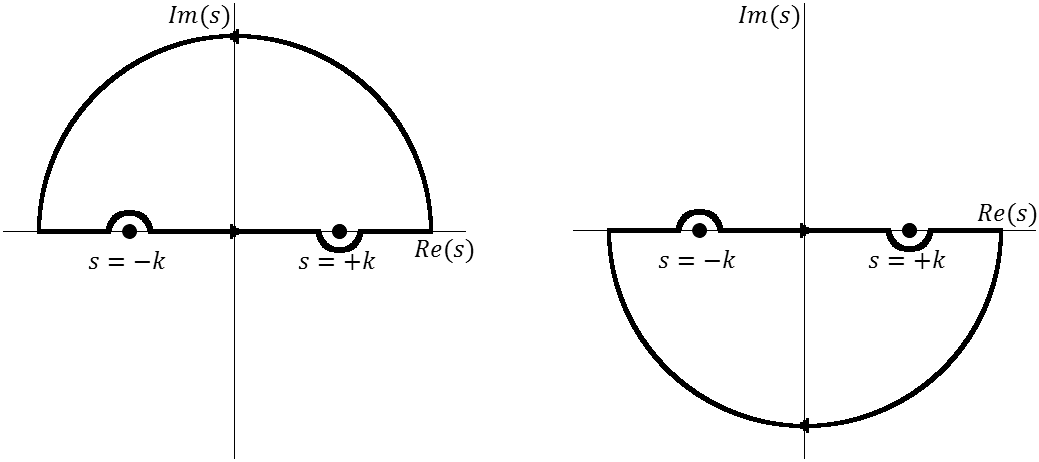
\includegraphics[width=\textwidth]{Figures/complexgreen} 
  \caption{Two parts of Green's function with their poles at $s=\pm k$, altered to be closed by a semicircle at $|s|=\pm\infty$.}
  \label{fig:complexgreen}
\end{figure}

Observe that in Eq. \eqref{eqn:complexgreen} the path integrals at $|s|=\pm\infty$ have been left out. This is because they do not contribute to the integral since the first integrand corresponds to the left side of Figure~\ref{fig:complexgreen} and goes like $e^{isr}$, hence going to zero at large positive imaginary numbers. Similarly, the second integrand goes like $e^{-isr}$ and goes to zero at large negative imaginary numbers.

Combining Eqns. \ref{eqn:cauchy} and \ref{eqn:complexgreen}, it can be seen that
%
\begin{equation}
\nonumber
G(\vec{r})=\frac{i}{8\pi^2r}[(i\pi e^{ikr})-(-i\pi e^{ikr})]=-\frac{e^{ikr}}{4\pi r}.
\end{equation}
This is a particular solution to the inhomogeneous Helmholtz equation. To get a general solution, the solution to the homogeneous Helmholtz equation must be added:
%
\begin{equation}
\label{eqn:greensolution}
G(\vec{r})=G_0(\vec{r})-\frac{e^{ikr}}{4\pi r};
\end{equation}
that is, $G_0(\vec{r})$ solves $(\nabla^2+k^2)G_0(\vec{r})=0$.

Using Eq. \eqref{eqn:psigreen} in conjunction with Eq. \eqref{eqn:greensolution} gives rise to the \emph{integrated} time-independent Schr\"{o}dinger equation:
%
\begin{equation} \label{eqn:integratedschrodinger}
\psi(\vec{r})=\psi_0 (\vec{r})-\frac{m}{2\pi\hbar^2}\int\frac{e^{ik|\vec{r}-\vec{r}_0|}}{|\vec{r}-\vec{r}_0|}V(\vec{r}_0)\psi(\vec{r}_0)d^3\vec{r}_0.
\end{equation}
%
That is, nothing has been said about the potential and so this equation is quite general. Eq. \eqref{eqn:integratedschrodinger} gives the recursive form for $\psi$. Let $g=-me^{ik|\vec{r}-\vec{r}_0|}/2\pi\hbar^2|\vec{r}-\vec{r}_0|$. Then Eq. \eqref{eqn:integratedschrodinger} says that
%
\begin{equation} \nonumber
\psi=\psi_0+\int gV\psi = \psi_0+\int gV (\psi_0+\int gV\psi).
\end{equation}
%
Applying this recursion several times gives the Born series:
%
\begin{equation}\nonumber
\psi=\psi_0+\int gV\psi_0+\int \int gVgV\psi_0 + \int \int \int gVgVgV\psi_0 + ...
\end{equation}
%
The zeroth term is exact if there is no scattering whatsoever (i.e. $V=0$) and the first term is accurate if the scattering potential is ``weak'' (that is, if $V$ is small enough for the second term to be neglected). For the purposes of this derivation, first order is a sufficient approximation for $\psi$. Then
%
\begin{equation} \nonumber
\psi=\psi_0+\frac{m}{2\pi\hbar^2}\int\frac{e^{ik|\vec{r}-\vec{r}_0}}{|\vec{r}-\vec{r}_0|}V(\vec{r}_0)\psi_0(\vec{r}_0) d^3\vec{r}_0.
\end{equation}

Recall that the strategy was to compare this solution of the Helmholtz equation with the wavefunction from the quantum scattering model (Eq. \eqref{eqn:scatteringwavefunction}) in order to find the scattering amplitude, $f(\theta)$. Doing so yields
%
\begin{equation} \nonumber
f(\theta)=-\frac{r}{e^{ikr}}\frac{m}{2\pi\hbar^2A}\int\frac{e^{ik|\vec{r}-\vec{r}_0|}}{|\vec{r}-\vec{r}_0|}V(\vec{r}_0)\psi_0(\vec{r}_0)d^3\vec{r}_0.
\end{equation}
%

The Coulomb potential goes as $1/r^2$, and as such $V(\vec{r}_0)$ is localized about $\vec{r}_0=0$. Since particles are observed far away from their scattering centers, it is advantageous to make use of the fact that $\vec{r} \gg \vec{r}_0$. However, caution must be taken, since one must evaluate the exponential and non-exponential terms separately, for they are of separate orders. For the non-exponential terms, this is simple, since
%
\begin{equation}\nonumber
\frac{r}{|\vec{r}-\vec{r}_0|}\approx1.
\end{equation}
%
The exponential terms look like
%
\begin{equation}\nonumber
e^{ik(|\vec{r}-\vec{r}_0|-r)},
\end{equation}
and so it is useful to expand the absolute value as
\begin{equation}\nonumber
|\vec{r}-\vec{r}_0|^2=r^2+r_0^2-2\vec{r}\cdot\vec{r}_0\approx r^2\left(1-2\frac{\vec{r}\cdot\vec{r}_0}{r^2}\right),
\end{equation}
%
or simply
%
\begin{equation} \nonumber |\vec{r}-\vec{r}_0|\approx r-\hat{r}\cdot\vec{r}_0. \end{equation}
%
This leaves
%
\begin{equation} \label{eqn:generalscattering}
f(\theta)=\frac{m}{2\pi\hbar^2}\int
e^{-ik\hat{r}\cdot\vec{r}_0}
V(\vec{r}_0)
e^{ik\hat{z}\cdot\vec{r}_0}
d^3\vec{r}_0,
\end{equation}
%
Now define $\vec{\kappa}\equiv k(\hat{z}-\hat{r})$ such that $\kappa=2k\sin{\theta/2}$. The exponential term becomes
%
\begin{equation} \nonumber
e^{i\vec{\kappa}\cdot\vec{r}_0}=e^{i\kappa r_0\cos{\theta_0}}.
\end{equation}
Furthermore, the form of the potential $V$ is known. Since the scattering for the low-$Z$ target happens at low temperatures, it is possible to use the Fermi-Thomas approximation for screening \cite{ashcroft}. This modifies the Maxwell equation 
\begin{align*}
\nabla^2 V(r) = -\frac{\rho}{\epsilon_0}
\end{align*}
to
\begin{equation} \nonumber
(\nabla^2-b^2)V(r)=-\frac{Q}{\epsilon_0}\delta(r),
\end{equation}
%
where $\rho$ is the charge density, $b$ is some screening constant, $\epsilon_0$ is the permittivity of free space, and $Q$ is the charge of the potential (in this case, the atomic number $Z$). The solution is
\begin{equation} \nonumber
V(r)=\frac{Q}{4\pi\epsilon_0}\frac{e^{-br}}{r}.
\end{equation}
Then the quantum scattering equation (Eq. \eqref{eqn:generalscattering}) becomes
%
\begin{equation} \nonumber
f(\theta)\propto \int e^{i\kappa r_0\cos(\theta_0)}e^{-br_0}r_0\sin(\theta_0)dr_0 d\theta_0 d\phi_0,
\end{equation}
where the amplitude terms have been left out since $|f(\theta)|^2$ is normalized anyway. Here it is seen that there does exist some $\theta$ dependence in $f(\theta)$ (by virtue of $\kappa$). The integral over $\phi_0$ is trivial, and the integral over $\theta_0$ can be done via $u$ substitution, with $u=\cos\theta_0$. This leaves
\begin{equation} \nonumber
f(\theta)\propto \frac{1}{\kappa}\int_0^\infty e^{-br_0}\sin(\kappa r_0) dr_0,
\end{equation}
%
which has the solution
\begin{equation}\nonumber
f(\theta)\propto\frac{1}{b^2+\kappa^2}.
\end{equation}
For classical Rutherford scattering, $b\rightarrow 0$. Recalling that $\kappa=2k\sin{\theta/2}$ yields the final Rutherford scattering distribution:
\begin{align}
|f(\theta)|^2 &\propto \frac{1}{\sin^4 \frac{\theta}{2}}=\frac{1}{\left(\sin^2 \frac{\theta}{2}\right)^2}=\frac{1}{\left(\frac{1}{2}\left[1-\cos^2\left(2\cdot\frac{\theta}{2}\right)\right]\right)^2},\nonumber \\
|f(\theta)|^2  &\propto\frac{1}{(1-\cos^2{\theta})^2}. \label{eqn:rutherford}
\end{align}

Only the tail of Eq. \eqref{eqn:rutherford} should be used since it blows up at $\theta=0$. This may seem like a contradiction since the Born series was truncated at the weak potential term (the first nontrivial term), and hence the incoming muons should not scatter much at all! In fact, the muons are not scattering much at all for each individual atom they encounter. Over the entire absorber, however, some muons have a net scattering angle which is small (and therefore should not be approximated by the Rutherford tail) whereas others have a large net scattering angle (and are well represented by Eq. \eqref{eqn:rutherford}). Many weak potentials can still induce a relatively large scattering angle.
